\documentclass[a4paper,twocolumn]{article}
\usepackage[a4paper,margin=2cm]{geometry} % Seitenränder anpassen
\usepackage{graphicx} % Für Grafiken
\usepackage{amsmath, amssymb} % Für mathematische Formeln
\usepackage{hyperref} % Für Hyperlinks
\usepackage{caption} % Für Bildunterschriften
\usepackage[printonlyused]{acronym}
\usepackage{pgffor} % Paket für die foreach-Schleife
\usepackage{shellesc} % Für das Ausführen von Shell-Befehlen (mit pdflatex -shell-escape)
\usepackage{todonotes}

% Abstand zwischen den Spalten erhöhen
\setlength{\columnsep}{1cm} 

\title{Augmented Reality with Aruco Markers}
\author{
    Hochschule Ravensburg-Weingarten \\[1em] % Hochschule zentriert
    \begin{minipage}[t]{0.45\textwidth} % Linke Spalte
        \centering
        Jonas Alber \\ % Name
        15444427\\
        \texttt{jonas.alber@hs-weingarten.de} % E-Mail
    \end{minipage}
    \hfill
    \begin{minipage}[t]{0.45\textwidth} % Rechte Spalte
        \centering
        Tim Schweitzer \\  29844429 \\ % Name
        \texttt{tim.schweitzer@hs-weingarten.de} % E-Mail
    \end{minipage}
}
\date{\today}

\begin{document}

\maketitle

\section*{Disclaimer}

The content of this document was created by the authors mentioned above. ChatGPT from OpenAI was used to improve readability. However, all content has been checked by the authors and adapted where necessary.


\section*{List of abbreviations}
\begin{acronym}[RWU]
    \acro{RWU}{Hochschule Ravensburg Weingarten}
    \acro{AI}{Artificial Intelligence}
    \acro{IoT}{Internet of Things}
\end{acronym}

\section{Introduction}

\subsection{Task definition}
This work was created as part of the Computer Vision course at \ac{RWU} as a project assignment. The aim of the project is to use the OpenCV library to modify images in such a way that a poster is integrated into the image in such a way that the viewer has the impression that the poster is actually in the room.
\\
This image augmentation is applied to a given data set, whereby the results obtained are then to be transferred to self-created images.
\subsection{Marker}
A central challenge in all computer science disciplines that work with image data is the interpretation of spaces on the basis of individual perspectives. One promising approach to recognizing orientation and alignment is the use of markers.
\\
The ArUco marker is used in this work. These are specially developed markers that consist of a square black and white pattern and enable clear identification and the calculation of position and orientation in space. \cite{aruco1}

\section{Image Transformation Process}
The image transformation process begins by loading the input image \ref{fig:example-base}, which contains ArUco markers, as well as the poster (Figure \ref{fig:img-poster}) image. 
\begin{figure}[h!]
    \centering
    \includegraphics[width=0.9\columnwidth]{img/img_base_113340.jpg} % Beispielbild
    \caption{Remote name of the Arucumarker from the previous data set.\cite{stefan-elser}}
    \label{fig:example-base}
\end{figure}
\\
The script then scales and adjusts the poster dimensions to fit within the area defined by the detected ArUco marker, ensuring the poster aligns properly with the marker's size and orientation. To achieve this, the script calculates the corners of the scaled poster and determines their correct positions relative to the marker's location. 
\\
Next, the ArUco markers are detected within the image using OpenCV's aruco.detectMarkers function, which identifies the marker's corners. A perspective transformation matrix is calculated based on the positions of the poster corners and the detected marker corners. This matrix is then used to warp the poster image so that it aligns precisely with the detected marker area.
\begin{figure}[h!]
    \centering
    \includegraphics[width=0.9\columnwidth]{img/detectedMarker_113340.jpg} % Beispielbild
    \caption{Detected Marker Image.\cite{stefan-elser}}
    \label{fig:detected-marker}
\end{figure}
\\
To integrate the transformed poster into the original image, a mask is created, which isolates the transformed poster region. 
The mask is then inverted so that only the region outside the poster area is kept, ensuring that the poster seamlessly blends with the background.
Finally, the mask is applied to the image, and the transformed poster is combined with the original image using bitwise operations, resulting in the final image with the poster placed correctly within the marker-defined region.

\section{Evaluation and Validation}

Once the image transformation is complete, the script proceeds to evaluate the alignment of the poster placement.
\begin{figure}[h!]
    \centering
    \includegraphics[width=0.9\columnwidth]{img/img_result_113340.jpg} % Beispielbild
    \caption{Remote name of the Arucumarker from the previous data set with poster.}
    \label{fig:example-result}
\end{figure}
 \\
 The first step in the evaluation is detecting the edges of the image using the Canny edge detection method. This process highlights the boundaries of the poster and the surrounding areas, providing a clear view of the poster's edges.
Following edge detection, the script employs the Hough Line Transform to extract the prominent lines from the edge-detected image. This method identifies and highlights the linear features within the image, including the edges of the poster. By comparing the detected lines with the expected positions of the poster's edges, the script can assess whether the poster has been placed accurately.
\\
Finally, the evaluation results are visualized by overlaying the detected lines and edges on the original image. This allows for easy manual inspection of the poster’s placement, providing immediate feedback on the transformation’s accuracy. The combination of edge detection and line extraction ensures that any misalignment or distortion in the poster placement is clearly visible for quality assurance.
\\
However, when analyzing further images, it becomes apparent that the detection of the Aruco marker does not work reliably in every perspective. An example of this is . Ein Beispiel hierfür ist in Abbildung \ref{fig:bad-example-result} zu sehen. Beim Vergleich der horizontalen Fluchtpunktlinien des Posters(Grün) mit der Metallstange(Rot) wird sichtbar, dass die Fluchtpunktlinien mit zunehmender Entfernung immer weiter von der Stange abweichen und schließlich abweichen.
Apart from the vanishing point, the posters are consistent in terms of placement and aspect ratio and allow the posters to be inserted stably.
\begin{figure}[h!]
    \centering
    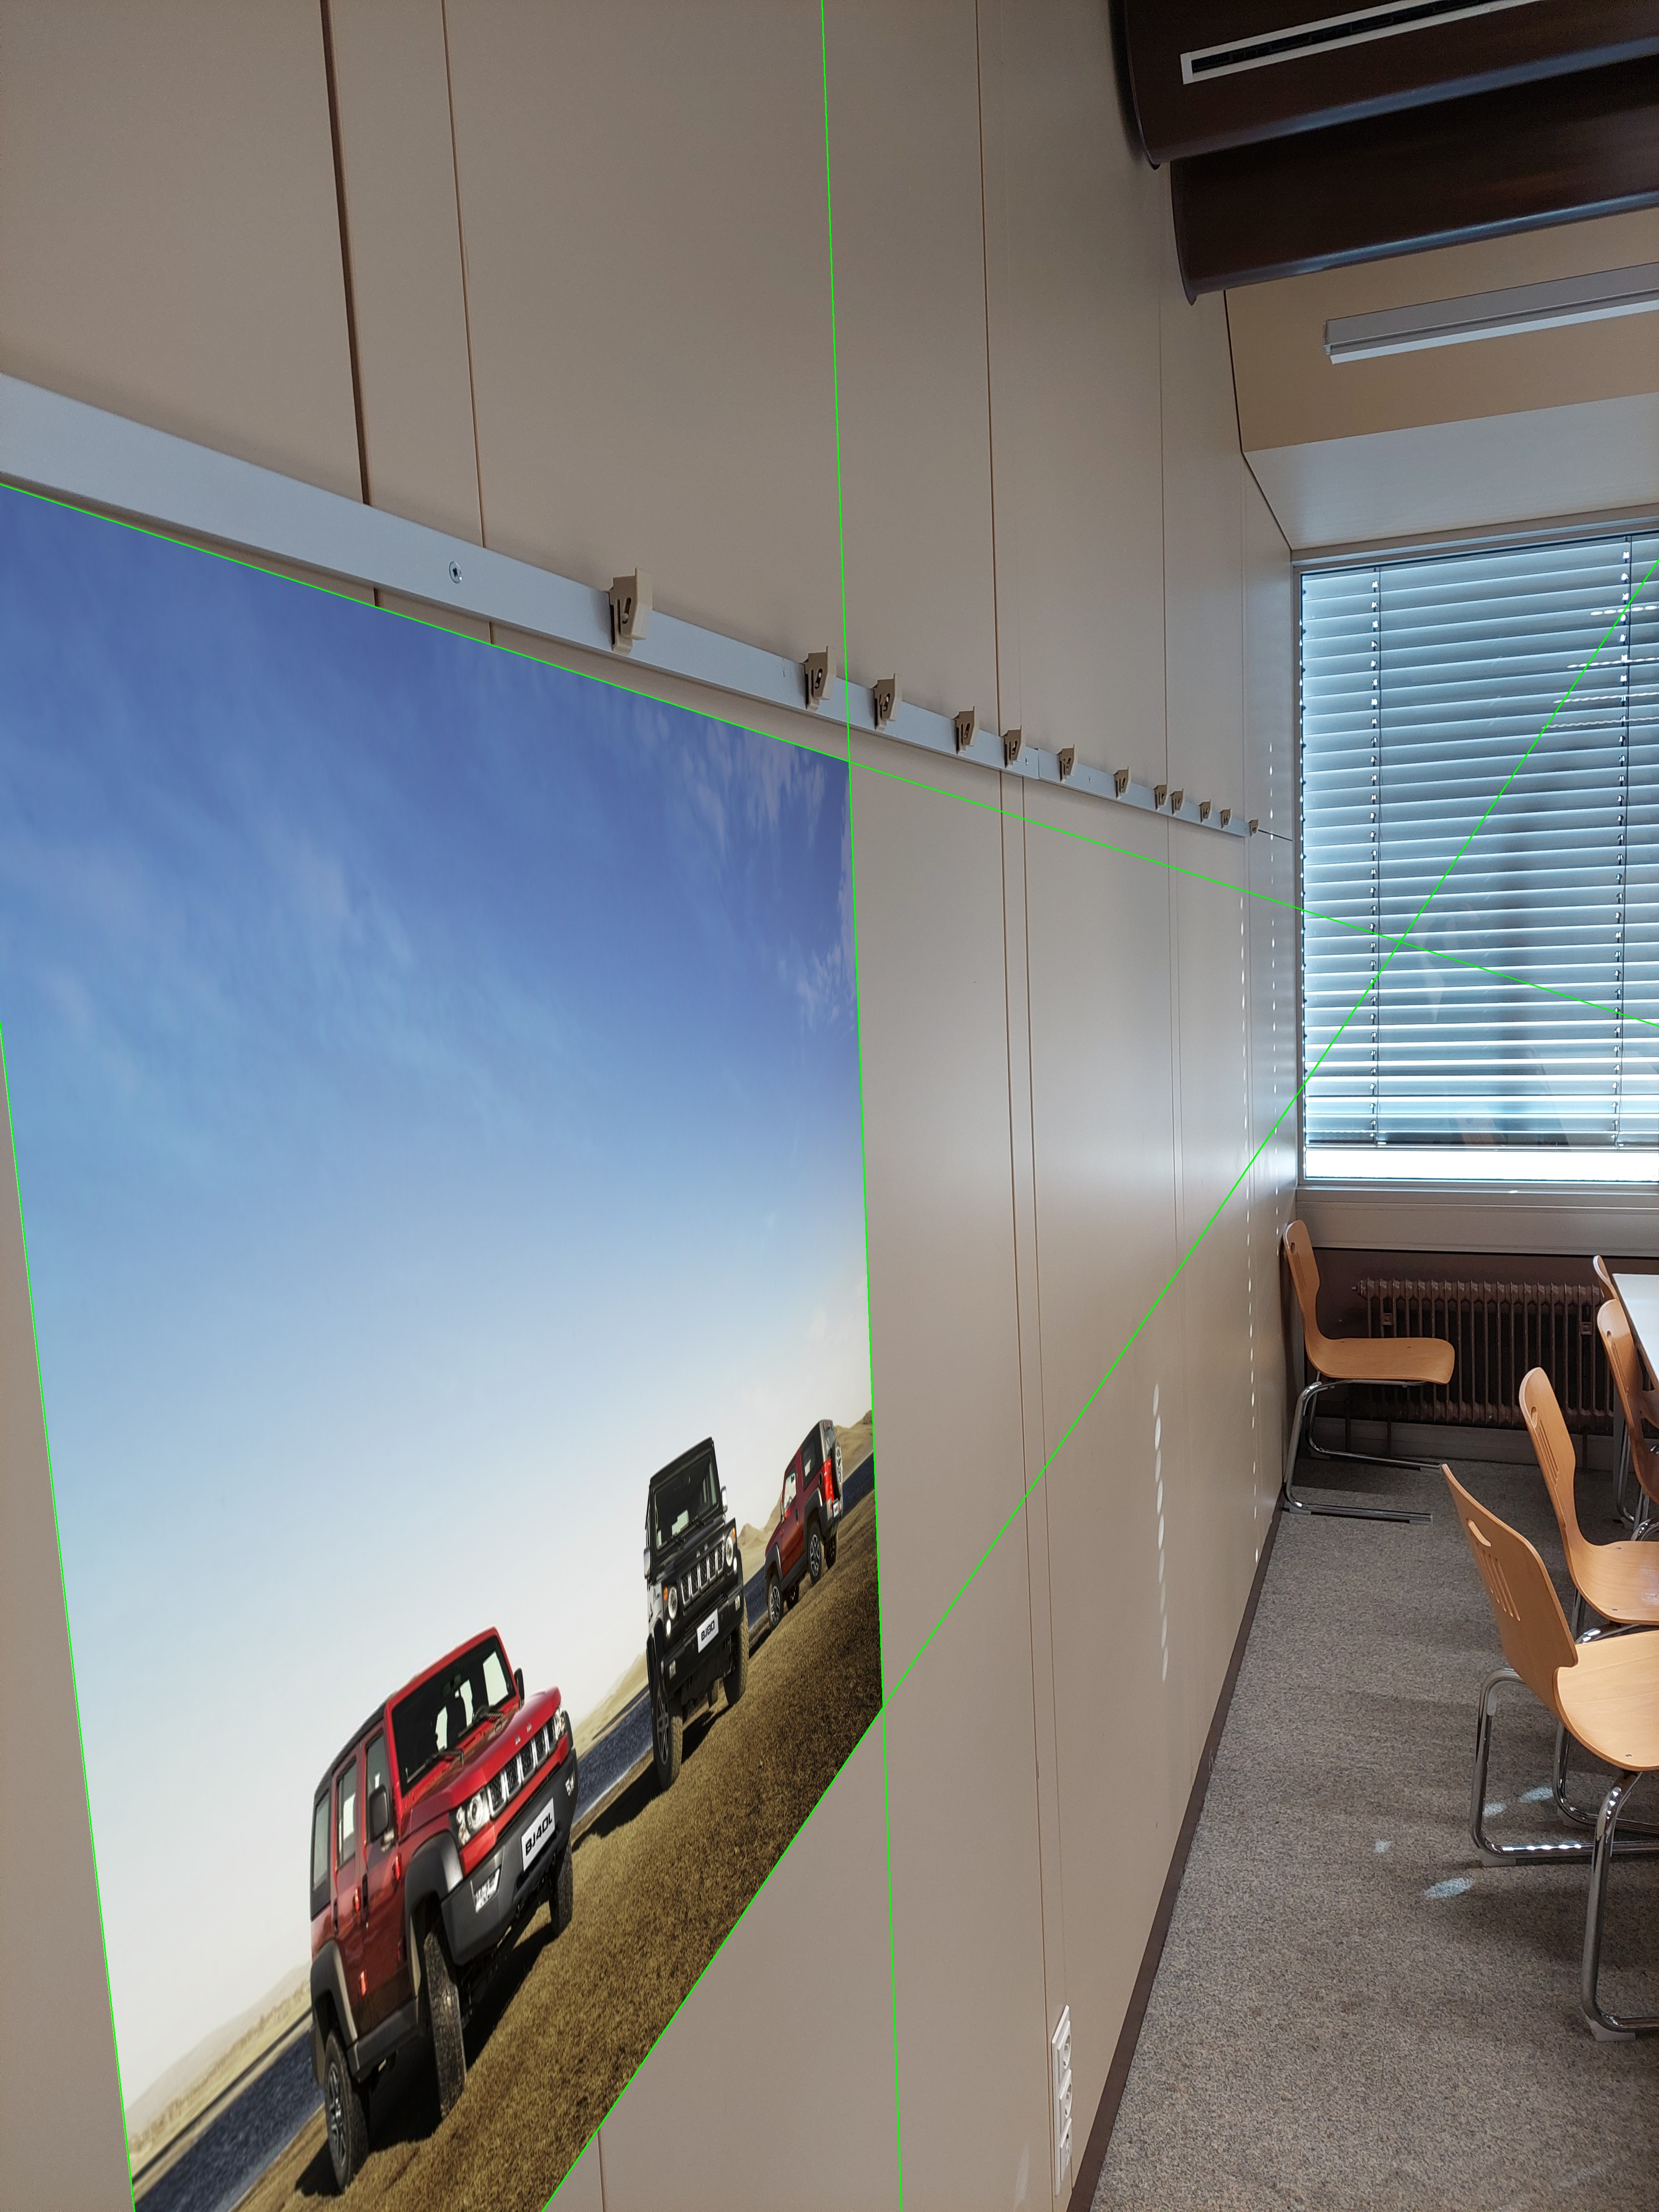
\includegraphics[width=0.9\columnwidth]{img/img_result_bad_113437.jpg} % Beispielbild
    \caption{Example of a perspective in which the vanishing point was poorly recognized.}
    \label{fig:bad-example-result}
\end{figure}

\section{Conclusion}
As part of this project, software for placing posters in an image was developed. The Aruco marker and the OpenCV library were mainly used for this.
\\
The results of the poster placement are basically solid and position the poster in the correct size in the room. The deviation between the calculated distortion and the actual distortion is
\\
An improvement of the marker detection was not possible within the scope of this work and could be further optimized in a more extensive scientific study.

%\end{document}
\begin{thebibliography}{9}

    \bibitem{aruco1}
    S. Garrido-Jurado, R. Muñoz-Salinas, F. J. Madrid-Cuevas, M. J. Marín-Jiménez. 
    \textit{Automatic generation and detection of highly reliable fiducial markers under occlusion}. 
    Pattern Recognition, vol. 11, no. 6, 2021.
    
    \bibitem{stackoverflow}
    \textit{Extract vanishing point from lines with OpenCV}, 
    StackOverflow user Ilke444. Available: \url{https://stackoverflow.com/questions/57535865/extract-vanishing-point-from-lines-with-open-cv}. 
    Accessed: Nov. 28, 2024.

    \bibitem{opencv}
    OpenCV.org, 
    \textit{Tutorial: ArUco detection}, 
    Available: \url{https://docs.opencv.org/4.x/d5/dae/tutorial_aruco_detection.html}. 
    Accessed: Nov. 28, 2024.

    \bibitem{tim-schweitzer}
    Tim Schweitzer \textit{Own example Images with Aruco Marker}, 2024.

    \bibitem{stefan-elser}
    Stefan Elser \textit{Image provided by Stefan Elser for this Project}, 2024.

    \bibitem{v_speed}
    v\_speed. \textit{Poster used in Images}, 2022. Available under Pixabay-Contentlicenz license: \url{https://pixabay.com/de/photos/beijing-automotive-bj40-suv-bj80-2486704/}. Accessed: November 3, 2024, 18:01.

\end{thebibliography}

\appendix
\section*{Appendix A: Additional Images}

\begin{figure}[h!]
    \centering
    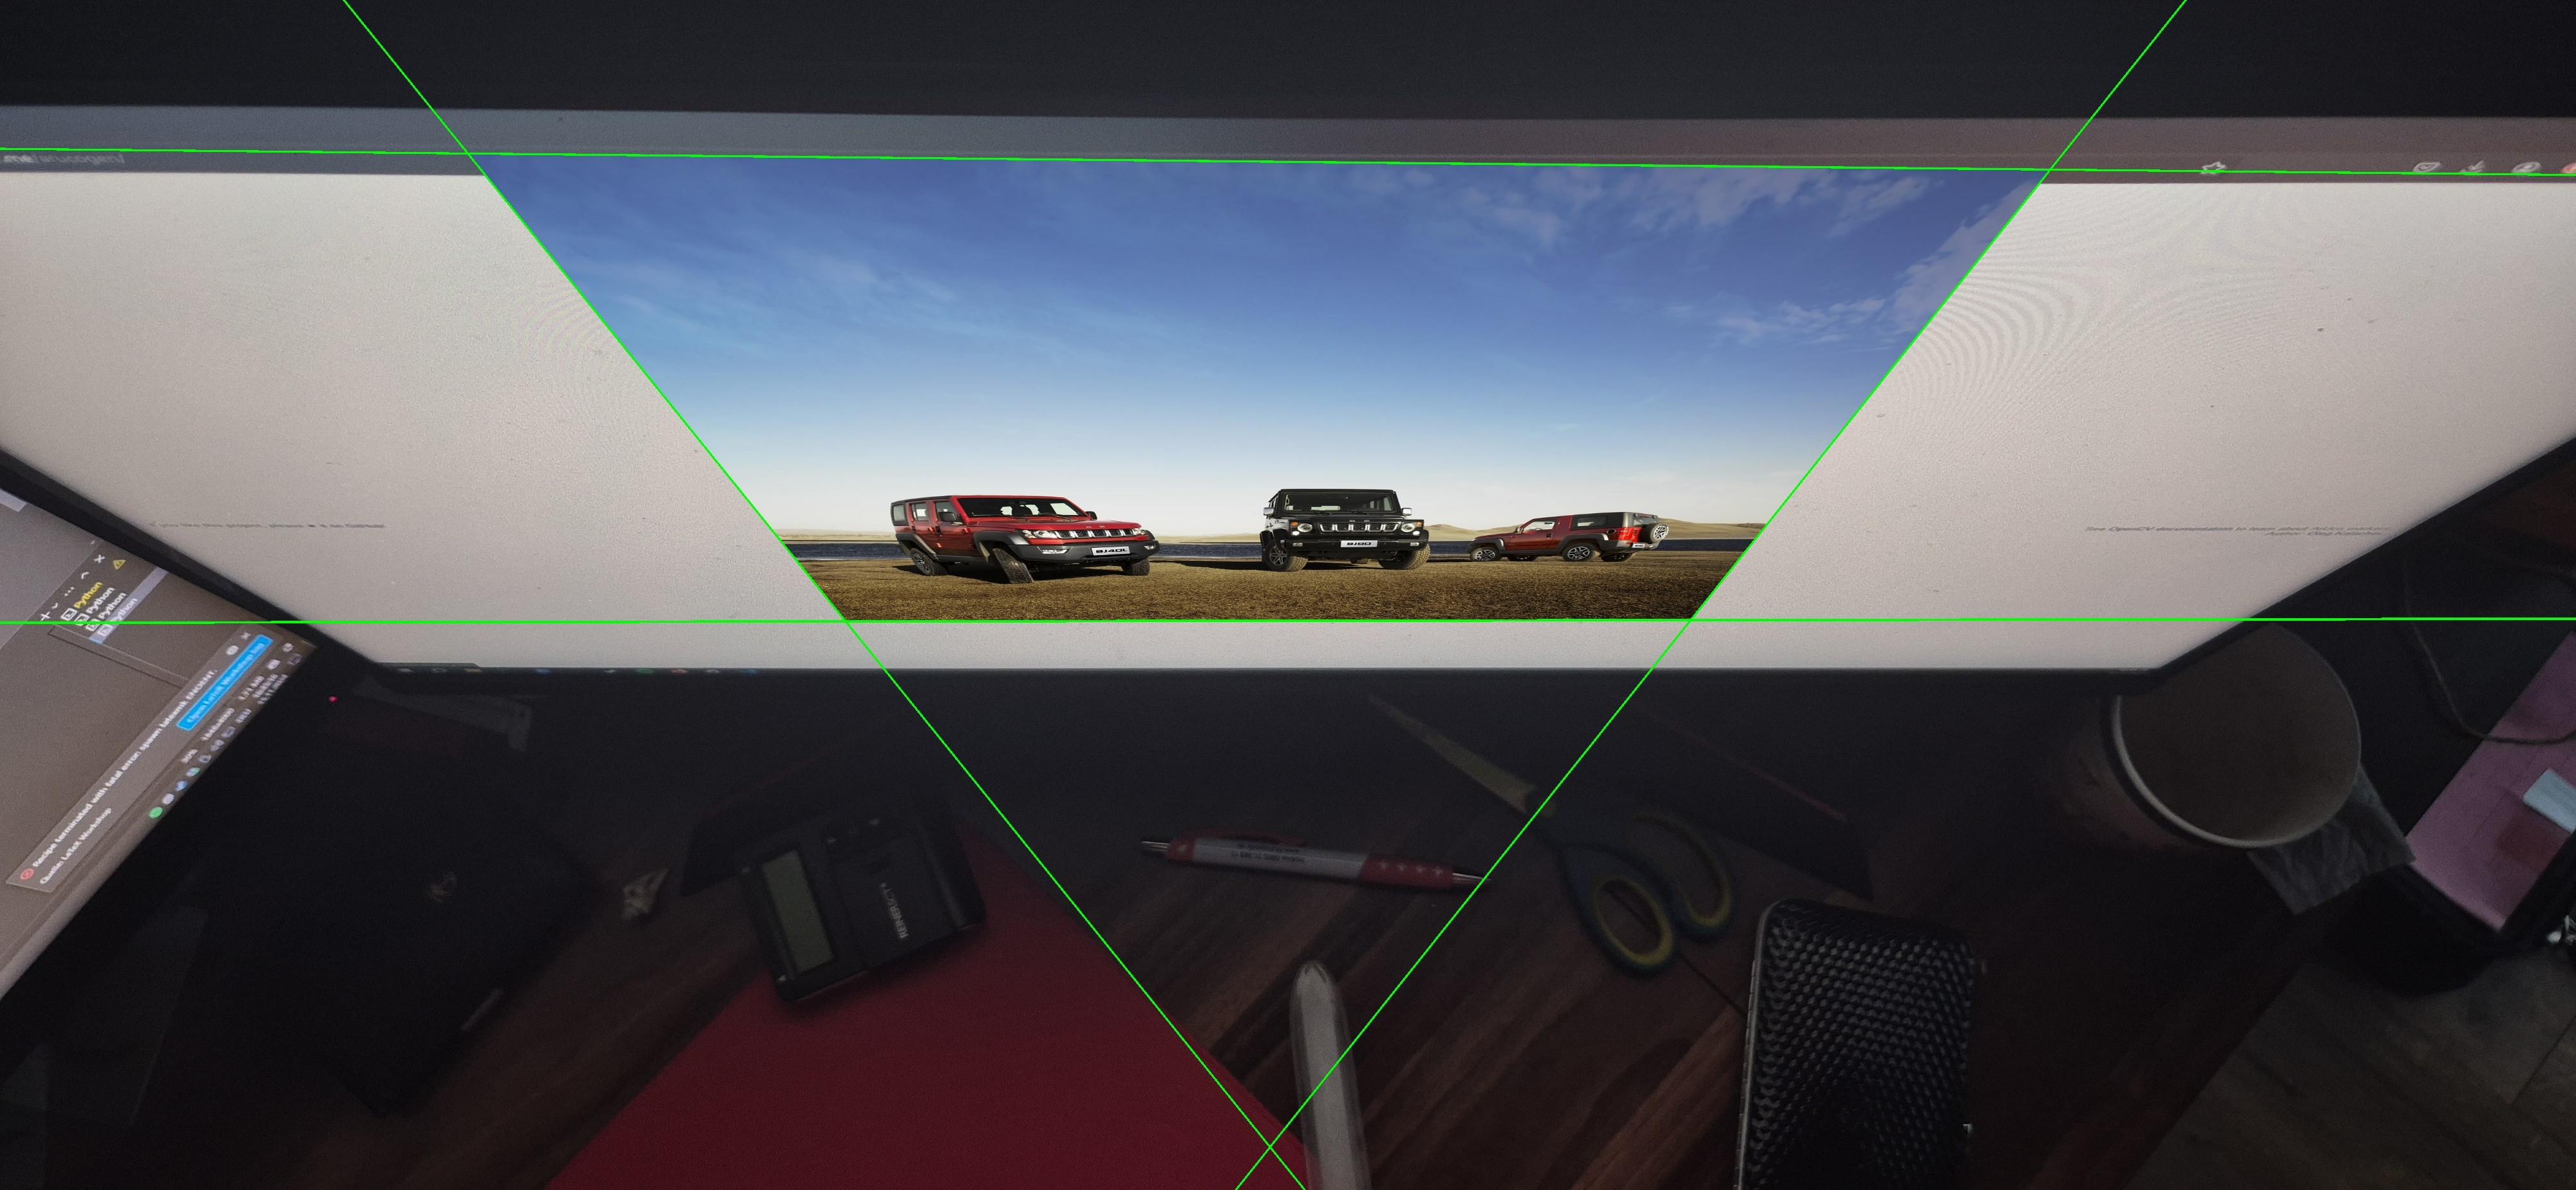
\includegraphics[width=0.9\columnwidth]{img_alt/aruco_from_screen.jpg}
    \caption{Aruco Marker on Screen \cite{tim-schweitzer}}
    \label{fig:example-appendix}
\end{figure}

\section*{Appendix B: Used Poster}

\begin{figure}[h!]
    \centering
    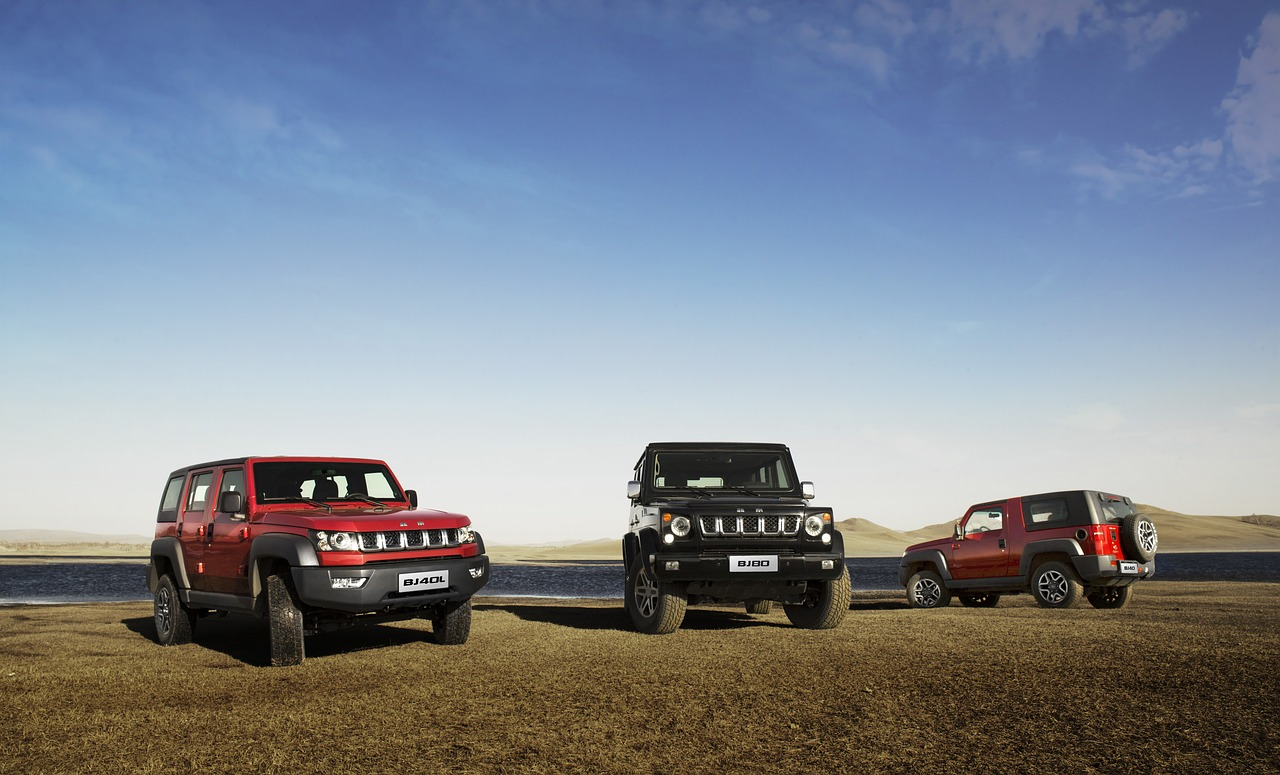
\includegraphics[width=0.9\columnwidth]{img_alt/poster.jpg}
    \caption{Poster used for Image Augmentation\cite{v_speed}}
    \label{fig:img-poster}
\end{figure}

\end{document}